
%(BEGIN_QUESTION)
% Copyright 2015, Tony R. Kuphaldt, released under the Creative Commons Attribution License (v 1.0)
% This means you may do almost anything with this work of mine, so long as you give me proper credit

\noindent
{\bf Labøvelse -- introduksjon}

\vskip 5pt

Oppgaven er å bygge, dokumentere og feilsøke et trykksmålesystem som består av en elektronisk $\Delta$P- eller overtrykksender koblet til en elektronisk indikator, skriver eller indikerende regulator. Instrumentlufttrykk, enten regulert eller uregulert, er anbefalt prosessvariabel å måle. Andre prosessvariabler kan også vurderes. Avvik fra standard laboppsett for trykkmåling krever godkjenning fra instruktør.

Tabellen under viser hva du og teamet må fullføre innen tidsrammen for denne labøvelsen.  Merk at noen av disse målene er individuelle, mens andre gjelder teamet som helhet:

\underbar{Tabell for måloppnåelse:}

% No blank lines allowed between lines of an \halign structure!
% I use comments (%) instead, so that TeX doesn't choke.

$$\vbox{\offinterlineskip
\halign{\strut
\vrule \quad\hfil # \ \hfil & 
\vrule \quad\hfil # \ \hfil & 
\vrule \quad\hfil # \ \hfil & 
\vrule \quad\hfil # \ \hfil & 
\vrule \quad\hfil # \ \hfil & 
\vrule \quad\hfil # \ \hfil & 
\vrule \quad\hfil # \ \hfil \vrule \cr
\noalign{\hrule}
%
% First row
{\bf Ytelsesmål} & {\bf Vurdering} & {\bf 1} & {\bf 2} & {\bf 3} & {\bf 4} & {\bf Team} \cr
%
\noalign{\hrule}
%
% Another row
Teammøte og prototypetegning (gjør dette {\it først!}) & mestring & -- & -- & -- & -- & \cr
%
\noalign{\hrule}
%
% Another row
Kretsdesignutfordring & mestring & & & & & -- -- -- -- \cr
%
\noalign{\hrule}
%
% Another row
Endelig sløyfediagram og systeminspeksjon & mestring & & & & & -- -- -- -- \cr
%
\noalign{\hrule}
%
% Another row
Digital trim (sensor og utgang) & mestring & -- & -- & -- & -- &  \cr
%
\noalign{\hrule}
%
% Another row
Ranging av sløyfe ($\pm$ 1\% av spennøyaktighet) & mestring & & & & & -- -- -- -- \cr
%
\noalign{\hrule}
%
% Another row
Forskning på og bruk av deadweight tester & mestring & & & & & -- -- -- -- \cr
%
\noalign{\hrule}
%
% Another row
Bruk av senderens ventilmanifold & mestring & & & & & -- -- -- -- \cr
%
\noalign{\hrule}
%
% Another row
Feilsøking & mestring & & & & & -- -- -- -- \cr
%
\noalign{\hrule}
%
% Another row
Labspørsmål: Instrumenttilkoblinger & proporsjonal &  &  &  &  & -- -- -- -- \cr
%
\noalign{\hrule}
%
% Another row
Labspørsmål: Idriftsetting & proporsjonal &  &  &  &  & -- -- -- -- \cr
%
\noalign{\hrule}
%
% Another row
Labspørsmål: Hoderegning & proporsjonal &  &  &  &  & -- -- -- -- \cr
%
\noalign{\hrule}
%
% Another row
Labspørsmål: Diagnostikk & proporsjonal &  &  &  &  & -- -- -- -- \cr
%
\noalign{\hrule}
%
% Another row
Nedstenging og opprydding i lab & mestring & -- & -- & -- & -- &  \cr
%
\noalign{\hrule}
} % End of \halign 
}$$ % End of \vbox

Den eneste ``proporsjonale'' vurderingen i denne aktiviteten er labspørsmålene, som besvares individuelt av hver student. En liste over mulige labspørsmål finnes mot slutten av oppgaven. Spørsmålene skal både styre arbeidet i laben og måle forståelsen din, og instruktøren kan derfor stille dem fortløpende gjennom perioden i stedet for samlet på én dag.

\vskip 10pt

{\bf Det er avgjørende at teamet planlegger på forhånd hva som skal gjennomføres hver dag. Et kort teammøte (10 minutter) i starten av hver labøkt er en god måte å gjøre dette på: gå gjennom hva som er gjort, hva som gjenstår, og hvilke vurderinger dere må være klare for. Det er mye arbeid knyttet til bygging, dokumentasjon og feilsøking av fungerende instrumentsystemer!}

Når du og teamet arbeider med systemet, vil dere uunngåelig møte problemer. Dere bør alltid forsøke å løse problemene som team før dere ber instruktøren om hjelp. Hvis dere fortsatt trenger hjelp, skriv teamfargen på labtavlen sammen med en kort beskrivelse av hva dere trenger hjelp til. Instruktøren vil deretter møte hvert team i den rekkefølgen de står på tavlen.

$$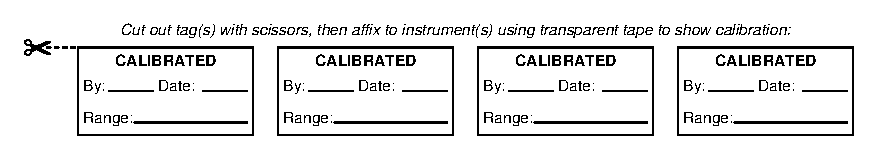
\includegraphics[width=15.5cm]{i00112x01.eps}$$





\vfil \eject

\noindent
{\bf Labøvelse -- teammøte, prototypetegning og instrumentvalg}

\vskip 5pt

Et viktig første steg i denne labøvelsen er å {\bf møte instruktøren} som team for å diskutere sikkerhet, teamytelse og konkrete roller for medlemmene. Hvis du ønsker mer erfaring med bestemt utstyr (for eksempel en bestemt type kontrollsystem eller spesifikke verktøy), teknikker (for eksempel mekanisk tilpasning) eller oppgaver for å styrke ferdighetene dine, er dette riktig tidspunkt å ta det opp med teamet.

\vskip 10pt

Et helt nødvendig steg i labøvelsen er å samarbeide som team for å {\bf skissere et prototypediagram} som viser hva dere skal bygge. Dette er vanligvis et enkelt koblingsskjema og/eller sløyfediagram som viser alle elektriske forbindelser mellom komponenter, samt rør- og slangeforbindelser for fluid. Prototypeskissen trenger ikke være ekstremt detaljert, men den må være tydelig nok til at instruktøren kan vurdere om alle komponenter blir riktig og sikkert koblet.

Hvis dere for eksempel skal koble feltutstyr til en PLS (programmable logic controller), må prototypeskissen vise hvordan disse enhetene kobles til typiske I/O-terminaler på PLS-en, hvor strømforsyning hentes fra osv. Skissen trenger ikke vise alle mellomforbindelser i detalj (for eksempel alle rekkeklemmer i hver koblingsboks), men den må være teknisk entydig.

Bruk gode problemløsningsmetoder når dere lager prototypeskissen: slå opp i manualer for komponentfunksjoner, marker strømretninger og polaritet, og identifiser kilder og laster. Se oppgaven som trening i analyseferdigheter. Husk at du senere skal kunne gjøre dette selvstendig (for eksempel i ``capstone''-vurderinger), så ikke gjør deg avhengig av at teamet løser alt for deg.

Teamets prototypeskisse er så viktig at instruktøren krever den før bygging kan starte. {\it Team som bygger uten godkjent plan vil bli stoppet til planen er ferdig og godkjent.} Dere skal heller ikke avvike fra godkjent design uten avklaring med instruktør, slik at utstyr ikke skades ved feil kobling. Alle på teamet bør ha enkel tilgang til planen gjennom hele byggeprosessen (helst egen kopi). Å lage prototypetegninger er en ferdighet og vane dere bør utvikle på skolen og ta med videre i yrkeslivet.

\vskip 10pt

Ved valg av feltinstrumenter til denne labøvelsen skal dere velge en {\it trykksender} med elektronisk signalutgang (4-20 mA), samt en ventilmanifold for å isolere senderen fra prosesstrykket. Se delkapittelet ``Valve manifolds'' i {\it Lessons In Industrial Instrumentation} for detaljer om utforming og bruk. Velg helst en sender med område mellom 10 PSI og 200 PSI. Unngå både lavområde-sendere (``draft'', få tommer vannsøyle) og høytrykksendere med områder på flere hundre eller tusen PSI.

Bruk dokumentasjon fra produsentens nettsted for å finne korrekt kobling, forsyning og kalibrering av senderen. Instruktøren vil kontrollere at dere har funnet og er kjent med relevant utstyrsdokumentasjon.

Etter at dere har funnet egnet instrument og dokumentasjon, skal instrumentet funksjonstestes før installasjon. For en trykksender betyr dette å påføre lufttrykk på ``high''-porten og måle mA-utgangen for å verifisere respons. Hvis senderen ikke reagerer korrekt, merk den tydelig med hva den gjør (eller ikke gjør).

\vskip 10pt

{\bf Planlegging av et fungerende system bør ikke ta mer enn én time ved effektivt teamarbeid, og vil spare dere for mange timer frustrasjon (og mulig komponentskade!).}








\vfil \eject

\noindent
{\bf Labøvelse -- kretsdesignutfordring}

\vskip 5pt

Koble et ``ice-cube''-relé til en lavspennings DC-kilde og 120 V AC slik at en håndbetjent bryter styrer innkobling av en 120 VAC-last. Alle elektriske koblinger skal utføres via rekkeklemmer (ingen tvinnede ledninger, klemhylseskjøter, ``wire nuts'', fjærklemmer eller krokodilleklemmer). 120 VAC-delen skal sikres mot overstrøm.

Denne øvelsen tester at du kan tolke pinout for et elektromekanisk relé, koble bryter korrekt til spolen, koble last korrekt til kontaktsettet, velge riktig NO/NC-kontakt både på bryter og relé, og organisere koblingene på en ryddig måte via rekkeklemmer.

$$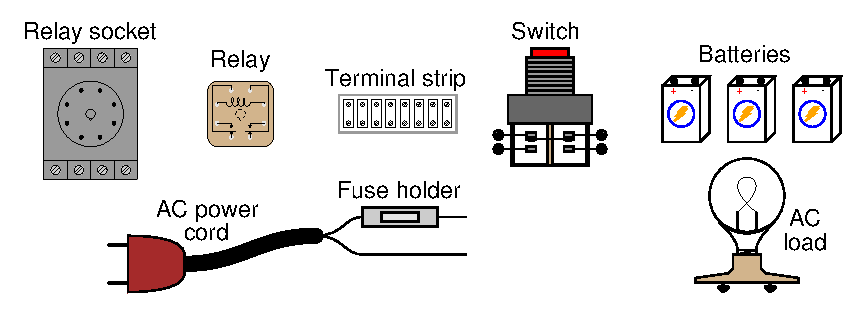
\includegraphics[width=15.5cm]{i00112x03.eps}$$

\vskip 10pt

Følgende komponenter og materiell er tilgjengelig: ulike ``ice cube''-{\bf reléer} med DC-spoler og tilhørende {\bf sokler} ; ulike trykknapp-{\bf brytere} ; {\bf rekkeklemmer} ; lengder med {\bf koblingstråd} ; {\bf batteriklemmer} (holdere) ; 120 VAC {\bf strømkabel} med {\bf sikringsholder} ; 120 VAC {\bf lampe eller annen egnet last}.

\vskip 10pt

Du forventes å bruke egne skrutrekkere og multimeter for montering og testing ved arbeidsplassen din. Instruktøren leverer batteri når kretsen er klar for funksjonstest. Fram til da skal kretsen være spenningsløs.

\vskip 20pt

\noindent
{\bf Last/bryterstatus} (instruktør velger): \hskip 20pt \underbar{\hskip 20pt} På ved trykk \hskip 10pt {\it eller} \hskip 10pt \underbar{\hskip 20pt} Av ved trykk

\vfil

Studiehenvisning: se seksjonen ``Control Relays'' i {\it Lessons In Industrial Instrumentation}.





\vfil \eject

\noindent
{\bf Labøvelse -- bygging av systemet}

\vskip 5pt

Instrumentlaben er satt opp for bygging av fungerende instrumentsløyfer, med mange koblingsbokser, ferdigtrukne signalkabler og stativer med 2-tommers vertikale rør for montering av instrumenter. De eneste ledningene dere normalt trenger å installere er mellom feltinstrument og nærmeste koblingsboks, samt korte ``jumper''-kabler mellom eksisterende kabler i mellomliggende bokser.

Etter at prototypeskissen er godkjent av instruktør, kan dere starte bygging. Sendere monteres på 2-tommers rør med egne braketter og U-bolter. Disse finnes sammen med senderne på instrumentlageret.

Velg en regulator som skal fungere som visning for målt trykk. Instruktøren kan velge regulator for teamet for å sikre bredere erfaring med ulike regulatorer.

Til slutt må trykksystemet få et unikt sløyfenummer, slik at instrumenter og kabler kan merkes riktig uten konflikt med andre team. En enkel metode er å bruke motstandsfargekoden for teamfargen som grunnlag for nummeret. For eksempel kan ``Rød''-team bruke sløyfenummer ``2''.

\vskip 10pt

{\bf Vanlige feil:}

\begin{itemize}
\item{} Å unnlate å bruke produsentdokumentasjon for feltinstrumenter (kobling, kalibrering).
\item{} Å montere feltinstrument i ugunstig posisjon, slik at terminaler og deksler blir utilgjengelige.
\item{} Feil montering av rør- og slangekoblinger (for eksempel blanding av gjenge- og kompresjonskoblinger).
\item{} Å ikke ettertrekke og dra-test hver leder i terminalpunktet.
\item{} At studenter jobber isolert uten å dele hva som er gjort; hele teamet må forstå hele systemet.
\end{itemize}

\vskip 10pt

{\bf Bygging av et fungerende system bør ikke ta mer enn én full labøkt (3 timer) hvis komponentene er tilgjengelige og teamet jobber effektivt!}





\vfil \eject

\noindent
{\bf Labøvelse -- dokumentasjon av systemet}

\vskip 5pt

Hver student må tegne sitt eget {\it sløyfediagram} for teamets system, i tråd med ISA-konvensjoner. Eksempler finnes i neste oppgave i dette arbeidsarket. Sløyfediagrammene må være {\it komplette} og {\it detaljerte}, med alle ledere, kabler, terminalpunkter, områdeverdier osv. Prinsippet er at dokumentasjonen skal være så tydelig at også personer uten forhåndskunnskap om anlegget kan følge koblingene korrekt.

Alle instrumenter og alle signalkabler i sløyfen skal merkes korrekt med ISA-standard tagnummer. En enkel metode er merketape rundt kabel og instrument, skrevet med permanent tusj. Selv om det ikke finnes én felles industristandard for kabelmerking, er en god praksis å merke hver toleder med tagnummeret til feltinstrumentet den går til. I en trykksløyfe merkes for eksempel kabler ``PT-$x$'', der ``$x$'' er sløyfenummer.

Når hele teamet er ferdig med individuelle sløyfediagram, tilkall instruktøren for inspeksjon av sløyfen. Teammedlemmene skal da gå gjennom sløyfen stegvis, mens de andre kontrollerer egne diagram for feil og mangler. Instruktøren vurderer samtidig installasjonskvalitet (for eksempel avisolering, terminalkvalitet, kabelføring, merking og deksler). Alle påpekte feil må rettes for å få godkjent.

Etter bestått inspeksjon skal hvert teammedlem legge sløyfediagrammet i diagramholderen midt i laben bak hovedpanelet. Ved senere feilsøking på andre team sine systemer hentes dokumentasjon herfra.

\vskip 10pt

{\bf Vanlige feil:}

\begin{itemize}
\item{} Å glemme merking av alle signalledere.
\item{} Å glemme merking av alle feltinstrumenter med korrekt tag (for eksempel PT-83).
\item{} Å utelate lederfarger i dokumentasjonen.
\item{} Å glemme navn på eget sløyfediagram.
\item{} Å kopiere fra et annet teammedlem i stedet for å kontrollere systemet selv.
\item{} Feil orientering av instrumenter på sløyfeark (feltinstrumenter til venstre, kontrollrominstrumenter til høyre).
\end{itemize}

\vskip 10pt

{\bf Å lage og kontrollere nøyaktige sløyfediagram bør ikke ta mer enn én full labøkt (3 timer) ved effektivt teamarbeid!}





\vfil \eject

\noindent
{\bf Labøvelse -- instrumentkalibrering}

\vskip 5pt

Hvert team skal kalibrere senderen (trim av både sensor og utgang) for å sikre korrekt trykktolkning og korrekt strømsignal. Deretter skal hvert teammedlem sette et eget måleområde (LRV/URV) og skalere indikator/regulator i riktige enheter. Instruktøren verifiserer nøyaktigheten ved å påføre tilfeldige trykk og sammenligne med vist verdi.

Som ved all kalibrering må responsen kontrolleres mot én eller flere {\it referansestandarder}. I denne øvelsen er en {\it presisjonstrykkmåler} (mekanisk eller elektronisk) egnet for inngangstrykk, mens et {\it multimeter} i mA DC-modus brukes for utgangssignal.

$$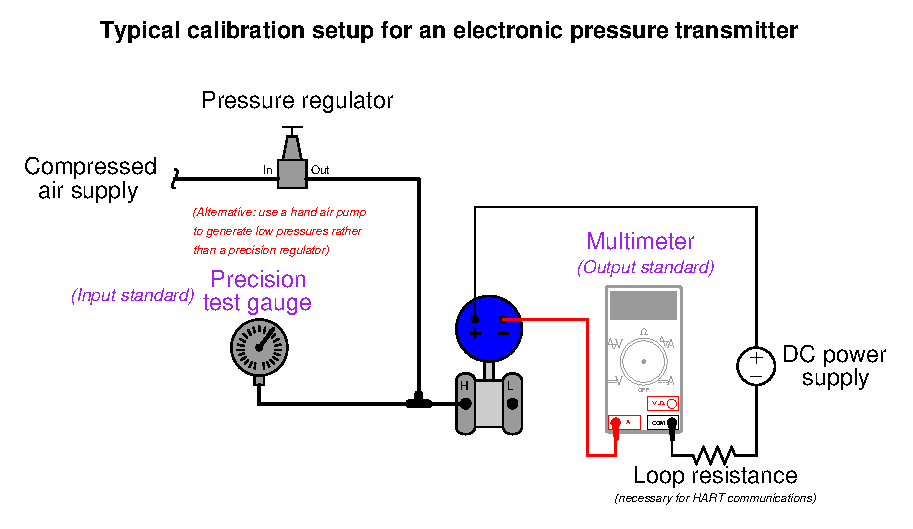
\includegraphics[width=15.5cm]{i00112x02.eps}$$

Forskjellen mellom ``kalibrering'' og ``ranging'' skaper ofte forvirring. I eldre {\it analoge} sendere var dette i praksis samme prosess. I moderne {\it digitale} instrumenter er det to separate oppgaver: kalibrering (trim mot kjent referanse) og ranging (definere 0\%- og 100\%-punkter i måleområdet).

\filbreak

Dokumenter nøyaktigheten til senderens sensortrim før og etter justering i tabellene under, ved fem ulike punkter i måleområdet:

\vskip 10pt

{\bf As-Found kalibreringstabell}

% No blank lines allowed between lines of an \halign structure!
% I use comments (%) instead, so that TeX doesn't choke.

$$\vbox{\offinterlineskip
\halign{\strut
\vrule \quad\hfil # \ \hfil & 
\vrule \quad\hfil # \ \hfil & 
\vrule \quad\hfil # \ \hfil & 
\vrule \quad\hfil # \ \hfil \vrule \cr
\noalign{\hrule}
%
% First row
Påført trykk & Utgangssignal (faktisk) & Utgangssignal (ideelt) & Feil (\% av spenn) \cr
%
\noalign{\hrule}
%
% Another row
 &  &  & \cr
%
\noalign{\hrule}
%
% Another row
 &  &  & \cr
%
\noalign{\hrule}
%
% Another row
 &  &  & \cr
%
\noalign{\hrule}
%
% Another row
 &  &  & \cr
%
\noalign{\hrule}
%
% Another row
 &  &  & \cr
%
\noalign{\hrule}
} % End of \halign 
}$$ % End of \vbox

\vskip 10pt

{\bf As-Left kalibreringstabell}

% No blank lines allowed between lines of an \halign structure!
% I use comments (%) instead, so that TeX doesn't choke.

$$\vbox{\offinterlineskip
\halign{\strut
\vrule \quad\hfil # \ \hfil & 
\vrule \quad\hfil # \ \hfil & 
\vrule \quad\hfil # \ \hfil & 
\vrule \quad\hfil # \ \hfil \vrule \cr
\noalign{\hrule}
%
% First row
Påført trykk & Utgangssignal (faktisk) & Utgangssignal (ideelt) & Feil (\% av spenn) \cr
%
\noalign{\hrule}
%
% Another row
 &  &  & \cr
%
\noalign{\hrule}
%
% Another row
 &  &  & \cr
%
\noalign{\hrule}
%
% Another row
 &  &  & \cr
%
\noalign{\hrule}
%
% Another row
 &  &  & \cr
%
\noalign{\hrule}
%
% Another row
 &  &  & \cr
%
\noalign{\hrule}
} % End of \halign 
}$$ % End of \vbox

Når teamets sender er ferdig kalibrert, sett på kalibreringsetikett med område og dato. Et sett med etiketter vises her og kan klippes ut og festes på senderen:

$$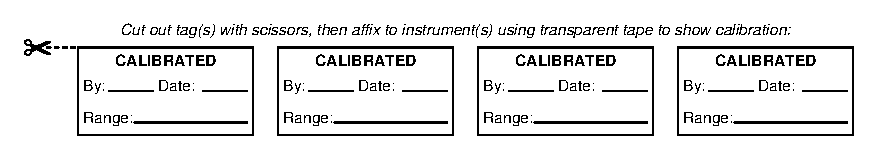
\includegraphics[width=15.5cm]{i00112x01.eps}$$

Hver student skal individuelt range sender og mottakende instrument (indikator/regulator/skrivende enhet). For digitale instrumenter gjøres dette typisk med HART-kommunikator eller programvareverktøy. Instruktøren verifiserer resultatet ved tilfeldige påførte trykk og kontroll av avlesning innen $\pm$ 1\% av spenn. Dette er også en god anledning til å demonstrere riktig bruk av ventilmanifold for å isolere senderen fra prosesstrykk.

\vskip 10pt

{\bf Vanlige feil:}

\begin{itemize}
\item{} Å ikke kontrollere regulatorporter før tilkobling av luftkilde.
\item{} Feil montering av rør/slangekoblinger.
\item{} Å velge for snevert trimområde i forhold til endelig måleområde.
\item{} Å bruke en referanse med for lav nøyaktighet til kalibrering.
\item{} Å glemme kalibreringsetikett etter trim.
\end{itemize}

\vskip 10pt

{\bf Trimming og individuell ranging av sender bør ikke ta mer enn én full labøkt (3 timer) ved effektivt teamarbeid!}







\vfil \eject

\noindent
{\bf Labøvelse -- bruk av deadweight tester}

\vskip 5pt

Deadweight-testere brukes for å generere kjente trykknivåer som referanse ved kalibrering av trykkinstrumenter. En del av labøvelsen er at hver student demonstrerer korrekt bruk av deadweight-tester for kontroll av kalibrering på trykkmåler. Flere deadweight-testere med olje som arbeidsmedium finnes i laben.

Informasjon om bruk finnes i {\it Lessons In Industrial Instrumentation}, på BTCInstrumentation sin YouTube-kanal og i produsentens dokumentasjon. {\it Du forventes å lese dette før bruk, og du blir muntlig spurt om innholdet.}

Når du er klar for demonstrasjon, skal instruktøren observere sikker påføring av trykk, samt forklaring av hvordan deadweight-testeren fungerer. Demonstrasjonen gjøres individuelt uten tilskuere.

\vskip 10pt

{\bf Vanlige feil:}

\begin{itemize}
\item{} Manglende forståelse av utstyrets funksjon før demonstrasjon.
\item{} Å ikke lufte ut systemet ved oppsett.
\item{} Å ikke gjenkjenne når stempelet står i endestopp.
\item{} Å unnlate å spinne vektene lett for å redusere statisk friksjon.
\item{} Å fjerne vekter mens trykk fortsatt er til stede.
\item{} Å stole mer på prosessmåler enn på deadweight-referansen.
\end{itemize}







\vfil \eject

\noindent
{\bf Labøvelse -- bruk av senderens ventilmanifold}

\vskip 5pt

En del av denne labøvelsen krever demonstrasjon av senderens {\it ventilmanifold}, enten 3-ventils eller 5-ventils. Dette innebærer praktisk håndtering av blokk-, equalizing- og bleed-ventiler i riktig rekkefølge, samt forklaring av hvorfor hvert steg utføres og hva senderen ``ser'' av trykk i hvert punkt.

Det anbefales sterkt å gjennomføre demonstrasjonen med lufttrykk på senderen, slik at feil blir synlige med en gang. For eksempel vil åpen bleed-port under åpning av blokkventil gi luftlekkasje. Øv på prosedyren selv før demonstrasjon for instruktør.

Informasjon om bruk av instrumentmanifolder finnes i {\it Lessons In Industrial Instrumentation}. {\it Som med deadweight-testeren forventes det at du leser dokumentasjonen før demonstrasjon.} Du skal kunne svare på grunnleggende spørsmål om funksjon og hensikt.

\vskip 10pt

{\bf Vanlige feil:}

\begin{itemize}
\item{} Å følge en memorert ventilsekvens uten å forstå hvorfor.
\item{} Å ikke øve individuelt før demonstrasjon.
\item{} Å ikke ta hensyn til retning på bleed-port av sikkerhetshensyn.
\item{} Forveksling av åpen/lukket retning på ventilhåndtak.
\end{itemize}









\vfil \eject

\noindent
{\bf Labøvelse -- feilsøking}

\vskip 5pt

Den mest krevende delen av labøvelsen er {\it feilsøking}, der du skal vise evne til logisk isolering av feil. Feilsøking vurderes individuelt (ingen teampoeng), og utføres på et system du ikke selv har bygget, slik at du må bruke sløyfediagram aktivt.

Hver student får 5 minutter til å identifisere både omtrent hvor feilen er og hva slags feil det er, med faglig begrunnelse for diagnostiske steg. Aktiviteten gjennomføres under direkte tilsyn av instruktør.

Dersom feilens plassering og type ikke identifiseres innen tiden, eller diagnostikken ikke er faglig begrunnet, underkjennes forsøket. Studenten må da prøve på nytt med en annen feil. Flere nye forsøk er tillatt uten karaktertrekk.

Standard multimeter er eneste tillatte testutstyr innen tidsgrensen. Bryting av krets for diagnostikk er kun tillatt etter godkjenning fra instruktør og med begrunnelse for konsekvenser i ekte anlegg.

Instruktøren går gjennom hvert feilsøkingsforsøk i etterkant og peker på styrker og svakheter. Feilsøking er en ferdighet som utvikles gjennom øving og feil, så flere forsøk er normalt.

\vskip 10pt

{\bf Vanlige feil:}

\begin{itemize}
\item{} Å unnlate å gjøre målinger med multimeter.
\item{} Å ikke sjekke støtteverdier i systemet (for eksempel manometeravlesning).
\item{} Feiltolkning av sløyfediagram ved valg av målepunkt.
\item{} Feil bruk av multimeter (AC/DC, område, probeplassering).
\end{itemize}

\vskip 10pt

{\bf Husk at formålet med feilsøkingsøvelsen er å utvikle og vurdere evnen til å diagnostisere komplekse systemer på en logisk måte. Treffer du feilen ved tilfeldighet, teller det ikke som faglig mestring.}

\vskip 10pt

{\bf Feilsøking krever mye labtid, ofte minst to økter á 3 timer i en full klasse. Planlegg deretter, og bruk muligheten til å observere andres feilsøking aktivt.}








\vfil \eject

\noindent
{\bf Labspørsmål}

\vskip 5pt

\begin{itemize}
\item{} {\bf Instrumenttilkoblinger}
\item{} Bestem korrekte lederkoblinger mellom instrumenter for en fungerende 4-20 mA-sløyfe, basert på terminalmerkede skjema.
\item{} Bestem korrekt hva som er kilder og laster, samt polaritet og strømretning i 4-20 mA-sløyfen.
\end{itemize}

\filbreak

\begin{itemize}
\item{} {\bf Idriftsetting og dokumentasjon}
\item{} Forklar hvordan en {\it tube fitting} tetter mot lekkasje, og hvordan dette skiller seg fra pipe fittings.
\item{} Forklar hvordan en konisk gjenget {\it pipe fitting} tetter mot lekkasje, og hvordan dette skiller seg fra tube fittings.
\item{} Forklar betydningen av {\it maximum working pressure} (MWP / maximum static pressure) og {\it maximum calibrated range} (LSL/USL) for en DP-sender.
\item{} Beskriv bruk av bleed-port-adapter (``stinger'') ved trykktest av DP-sender.
\item{} Forklar hva {\it turndown} ({\it rangedown}) betyr for en trykksender.
\item{} Forklar virkemåten til trykksenderen så detaljert som mulig.
\item{} Forklar valg av remote-seal-fyllvæsker for ulike prosesser (for eksempel oksygen, næringsmiddel, farmasi).
\end{itemize}

\filbreak

\begin{itemize}
\item{} {\bf Hoderegning} (uten kalkulator)
\item{} Beregn riktig sløyfestrøm (mA) gitt kalibreringsområde og påført trykk.
\item{} Beregn påført trykk gitt kalibreringsområde og målt sløyfestrøm.
\item{} Beregn prosentvis spennfeil gitt kalibreringsområde og As-Found-tabell.
\item{} Beregn tillatt trykkfeil gitt tillatt prosentvis spennfeil og kalibreringsområde.
\item{} Konverter mellom trykkenheter uten oppslag i tabeller.
\end{itemize}

\filbreak

\begin{itemize}
\item{} {\bf Diagnostikk}
\item{} Forklar hvordan ``åpen kabel'' skilles fra ``kortsluttet kabel'' med kun voltmeter.
\item{} Vurder om en foreslått diagnostisk test faktisk gir nyttig informasjon.
\item{} Oppgi minst to plausible feil gitt testresultater og symptomer.
\item{} Foreslå en diagnostisk test og forklar to mulige testutfall.
\end{itemize}




\vfil \eject

\noindent
{\bf Labøvelse -- nedstenging og opprydding}

\vskip 5pt

Siste steg i labøvelsen er å demontere teamets system og legge komponenter tilbake på riktig lagringsplass, slik at laben klargjøres for neste øvelse. Fjern egen dokumentasjon fra fellesområdet, fjern instrumentmerking fra instrumenter og kabler, og rydd arbeidsplassen fullstendig.

\vskip 10pt

\indent
{\bf La følgende komponenter stå montert på stativene:}

\begin{itemize}
\item{} Store reguleringsventiler og posisjonerere
\item{} I/P-transdusere
\item{} Store elektriske motorer
\item{} Store frekvensomformere (VFD)
\item{} Kabler i rør mellom koblingsbokser
\item{} Rør- og slangekoblinger (ikke demonter rørgjenger)
\item{} Regulatorer for forsyningsluft
\end{itemize}

\vskip 10pt

\indent
{\bf Returner følgende komponenter til riktig lagringsplass:}

\begin{itemize}
\item{} Følere/sensorelementer (for eksempel termoelementer, pH-prober)
\item{} Prosessendere
\item{} ``Jumper''-kabler mellom rekkeklemmer i samme koblingsboks
\item{} Plastslanger og slangekoblinger (koble fra kompresjonskoblinger)
\item{} Strømkabler og skjøteledninger
\item{} Justeringsregulatorer for luft (loading station)
\end{itemize}

\vskip 10pt

Til slutt skal alle kontrollsystemkomponenter settes tilbake til opprinnelig (fabrikkstandard) konfigurasjon, inkludert PID-parametere, funksjonsblokker og inngangsområder.



\underbar{file i00112}
%(END_QUESTION)





%(BEGIN_ANSWER)


%(END_ANSWER)





%(BEGIN_NOTES)

\noindent
{\bf Sløyfediagram / inspeksjon:}

Jeg anbefaler at du krysser av studentenes sløyfediagram samtidig som du inspiserer sløyfen sammen med teamet (mekanisk kvalitet, kabelføring, rørføring, osv.). La alle teammedlemmene forklare hver sin del av den ferdige sløyfen med eget sløyfediagram som støtte. Dette sparer tid og sikrer at de faktisk forstår sammenhengen mellom dokumentasjon og fysisk installasjon.

\vskip 10pt

\goodbreak

\noindent
{\bf Feilsøkingsforslag:}

\begin{itemize}
\goodbreak
\item{} Strip wire at terminal, then insert insulated wire end under terminal and tighten (open wire fault)
\item{} Cut signal cable somewhere in mid-conduit (open wire fault)
\item{} Push a thumbtack through the cable somewhere in mid-conduit (shorted wire fault)
\item{} Wire instrument cable conductors backward (construction fault)
\item{} Configure transmitter for excessive damping (slow response fault)
\item{} Configure indicator/controller for excessive damping (slow response fault)
\item{} Miscalibrate transmitter and/or indicator/controller (inaccuracy fault)
\item{} Plug tube connections using portion of foam earplug stuffed into tube fitting (slow response fault)
\item{} Reverse action of controller/positioner/transmitter (wrong response fault)
\item{} Mis-configure linear/sq.root characterization of transmitter and/or indicator/controller (nonlinearity fault)
\item{} Koble en 2.2 k motstand parallelt med 4-20 mA-sender for å simulere delvis kortslutning i kabling (nøyaktighetsfeil)
\item{} Exchange 250 ohm resistor for a different resistor that looks the same but has the wrong value (inaccuracy fault) 
\item{} Unplug cable(s) inside transmitter or controller (failed instrument fault)
\item{} Give students wrong sløyfediagram (documentation fault)
\item{} Close valve and leave safety tag hanging on it (operator/technician error)
\end{itemize}







\vfil \eject

\noindent
{\bf Labspørsmål}

\vskip 20pt

\begin{itemize}
\item{$(1)$} Sketch connecting wires necessary to make this loop-powered DP transmitter provide a signal to the controller's analog input \#2:

$$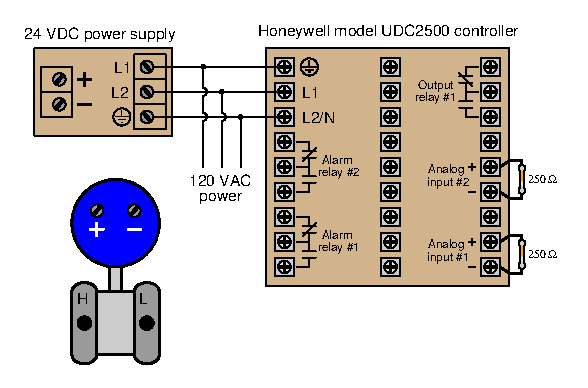
\includegraphics[width=15.5cm]{i00112x05.eps}$$

\vskip 20pt

\item{$(2)$} Forklar hensikten med {\it fyllvæske} i trykksenderens sensor.

\vskip 20pt

\item{$(3)$} Beregn feil i prosent av spenn for en trykksender med område 0 til 300 PSI når senderen viser 163 PSI ved faktisk påført trykk 175 PSI.

\vskip 20pt

\item{$(4)$} PIR-528 viser $-25$ "WC (``pegged'' lav) for prosessvariabel (PV). En instrumenttekniker måler 0 VDC mellom terminal 13 og 14. Identifiser \underbar{to} ulike feil som kan forklare symptomene, og vær så spesifikk som mulig.
\end{itemize}

$$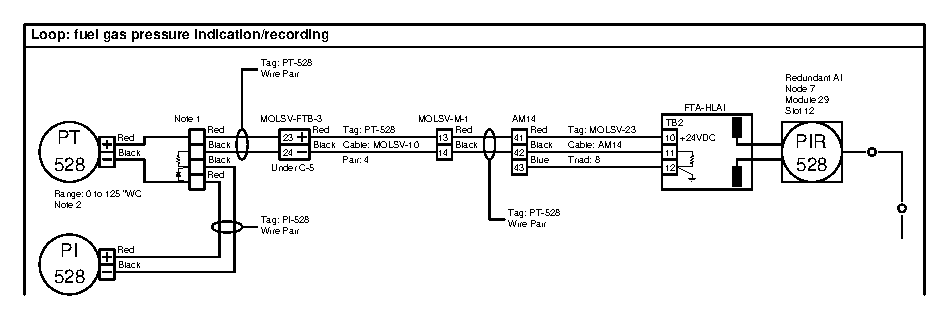
\includegraphics[width=15.5cm]{i00112x04.eps}$$








\vfil \eject

\noindent
{\bf Labspørsmål}

\vskip 20pt

\begin{itemize}
\item{$(1)$} Sketch connecting wires necessary to make this loop-powered DP transmitter provide a signal to the controller's analog input \#1:

$$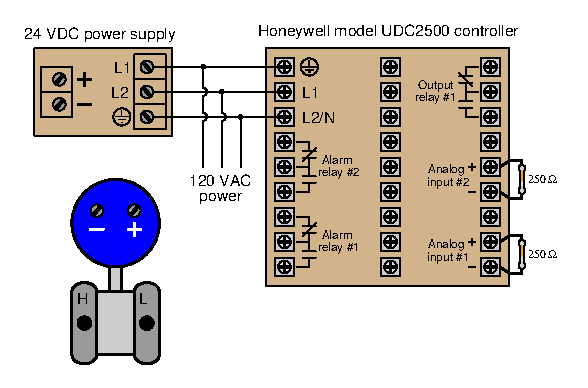
\includegraphics[width=15.5cm]{i00112x06.eps}$$

\vskip 20pt

\item{$(2)$} Identifiser og forklar {\it maximum working pressure} (MWP, også kalt ``maximum static pressure'') for trykksenderen, og hvordan denne skiller seg fra {\it maximum calibrated range} (LSL/USL).

\vskip 20pt

\item{$(3)$} Beregn tillatt trykkfeil for en trykksender med område 0 til 250 PSI og tillatt spennfeil på $\pm$ 0.5\%.

\vskip 20pt

\item{$(4)$} PIR-528 viser 133 "WC (``pegged'' høy) for prosessvariabel (PV). En instrumenttekniker måler 0 VDC mellom terminal 13 og 14. Identifiser \underbar{to} ulike feil som kan forklare symptomene, og vær så spesifikk som mulig.
\end{itemize}

$$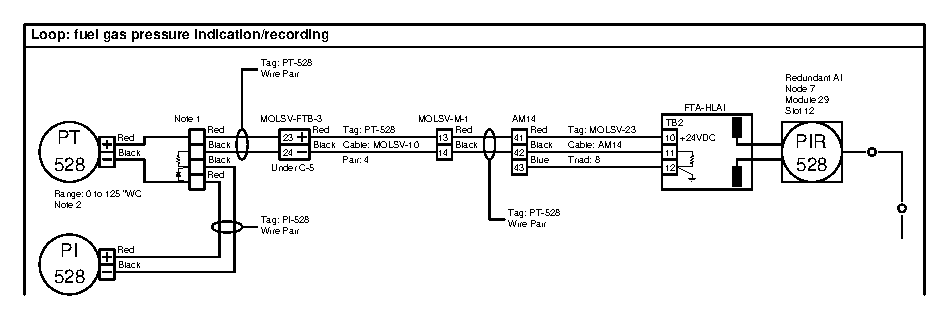
\includegraphics[width=15.5cm]{i00112x04.eps}$$


%INDEX% Lab exercise, deadweight tester
%INDEX% Lab exercise, electronic DP transmitter
%INDEX% Lab exercise, pressure measurement loop

%(END_NOTES)
